\documentclass[a4j]{jarticle}
\usepackage[dvipdfmx]{graphicx}
\usepackage{here}
\usepackage{ascmac}
\usepackage{url}
\title{
\vspace{30mm}
株式会社マルナカ様\\
購入商品情報管理システム\\
内部設計書v1.0
\vspace{90mm}
}
\author{
株式会社Toron
}

\begin{document}
\maketitle
\newpage
\tableofcontents
\newpage
\section{コーディング規約}

本節では本システムを開発する際のコーティング規約を示す。また、命名規則として英単語を使用する。
\subsection{Java}

本小節ではJavaを使用する際のコーディング規約を示す。1レベルインデントするごとに半角空白を4つ使用する。
\begin{itemize}
	\item クラス\\
		クラス名にはアッパーキャメルケース表記を使用する。
	\begin{itemize}
		\item 2つ以上の英単語を使用する
		\item 単語の頭文字は大文字を使用する
		\item 名称には英字のみを使用する
	\end{itemize}
		クラスの役割に応じて表 \ref{tab:o1} に示す単語を名称の最後に使用する。
		%
		\begin{table}[H]
			\caption{Javaのクラス名に使用する単語}
			\label{tab:o1}
			\begin{center}
			\begin{tabular}{|c|c|}
			\hline
			画面定義 & Activity\\\hline
			\end{tabular}
			\end{center}
			\end{table}
	\item メソッド\\
		メソッド名にはアッパーキャメルケース表記を使用する。
	\begin{itemize}
		\item 2つ以上の英単語を使用する
		\item 単語の頭文字は大文字を使用する
		\item 名称には英字のみを使用する
	\end{itemize}
		メソッドの実装に応じて表 \ref {tab:o2} に示す単語を名称の最初に使用する。
		%
				\begin{table}[H]
			\caption{Javaのメソッド名に使用する単語}
			\label{tab:o2}
			\begin{center}
			\begin{tabular}{|c|c|}
			\hline
			データの取得 & Get\\\hline
			データの設定 & Set\\\hline
			データの表示 & Display\\\hline
			データの並び替え & Sort\\\hline
			データの更新  & Updata\\\hline
			データの削除  & Delete\\\hline
			データの照合 & Check\\\hline
			\end{tabular}
			\end{center}
			\end{table}
	\item 変数・定数\\
		変数名または定数名にはアッパーキャメルケース表記を使用する。
	\begin{itemize}
		\item 2つ以上の英単語を使用する
		\item 単語の頭文字は大文字を使用する
		\item 名称には英字のみを使用する
	\end{itemize}


\end{itemize}
\subsection{Javascript}

本小節ではJavascriptのコーディング規約を示す。

\begin{itemize}
	\item メソッド\\
		メソッド名にはアッパーキャメルケース表記を使用する。
	\begin{itemize}
		\item 2つ以上の英単語を使用する
		\item 単語の頭文字は大文字を使用する
		\item 名称には英字のみを使用する
	\end{itemize}
		メソッドの実装に応じて表 \ref {tab:o3} に示す単語を名称の最初に使用する。
				\begin{table}[H]
			\caption{Javascriptのメソッド名に使用する単語}
			\label{tab:o3}
			\begin{center}
			\begin{tabular}{|c|c|}
			\hline
			データの取得 & Get\\\hline
			データの設定 & Set\\\hline
			データの更新  & Updata\\\hline
			データの削除  & Delete\\\hline
			\end{tabular}
			\end{center}
			\end{table}
	\item 変数・定数\\
		変数名または定数名にはローワーキャメルケース表記を使用する。
	\begin{itemize}
		\item 2つ以上の英単語を使用する
		\item 名称の頭文字は小文字を使用し、後続する単語の頭文字は大文字を使用する
		\item 名称には英字のみを使用する
	\end{itemize}
\end{itemize}
\subsection{データベース}
本小節ではデータベースのコーディング規約を示す。
	\begin{itemize}
	\item 共通\\
		スネークケース表記を使用する。
	\begin{itemize}
		\item 使用する文字は全て大文字とする
		\item 単語が連なる場合は後続する単語の前にアンダースコアを使用する
	\end{itemize}
	\item テーブル\\
		変数名または定数名にはローワーキャメルケース表記を使用する。
	\item カラム
		主キーの名称はテーブル名、アンダースコア、idで命名する。
\end{itemize}


\section{モジュール設計(Webページ)}

本節ではWebページのモジュール設計を示す。また、本システムで用いるサーバのディレクトリ構造を図\ref {tab:oonishimoj}に示す。

\begin{figure}[H]
\begin{center}
\resizebox{16cm}{!}{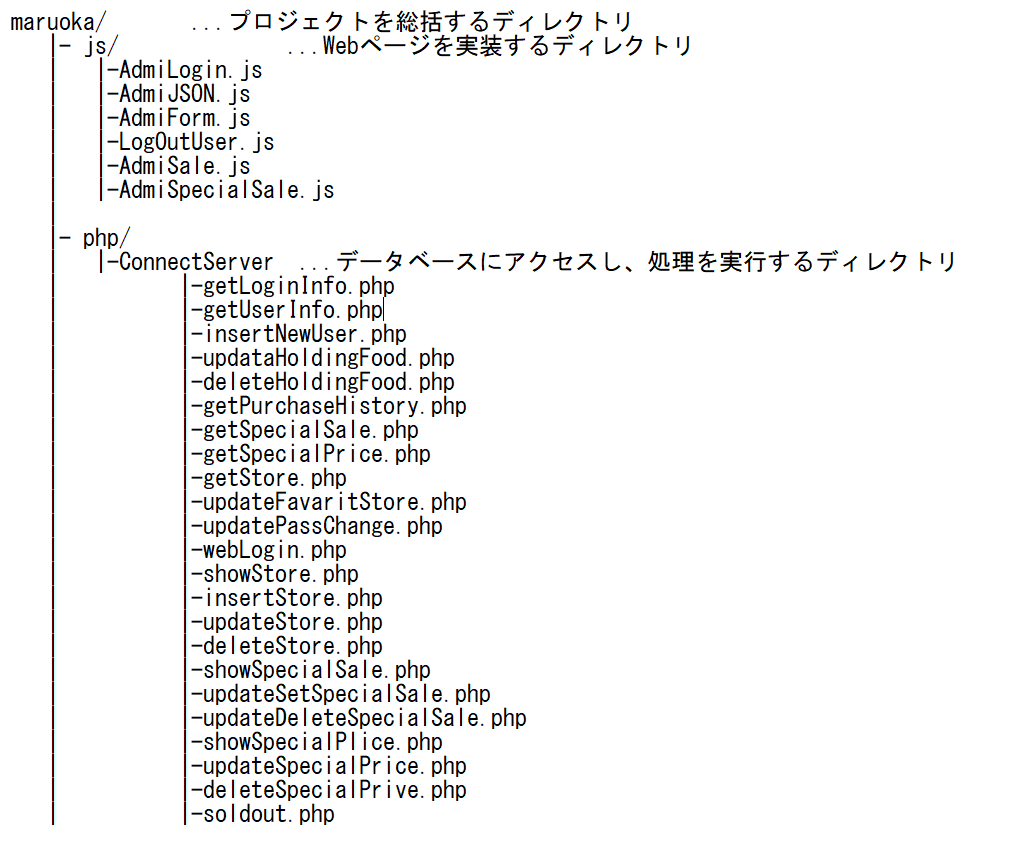
\includegraphics{webmoj.PNG}}
\caption{モジュール構成図}
\label{tab:oonishimoj}
\end{center}
\end{figure}
\subsection{管理者ページmaruokaディレクトリ}
webに関するすべての機能に関連するファイルが設置されているディレクトリである。\\
本小節では内包されている各ファイルについて示す。
\subsubsection{AdmiLogin.js}
ログイン画面を提供し、ユーザ情報に伴いページの遷移を行うクラスである。
\begin{itemize}

\item メソッド名:AuthentivationUsed\\

Webページでログインする際に、入力されたログイン情報がデータベースに登録されているか問い合わせを行うメソッドである。\\
引数として、入力されたユーザIDとパスワードを受け取る。\\
また返り値はIdentifivationNumberである。これは、データベース上にログイン情報が存在したか判定を行った結果を返すものである。\\

	\begin{itemize}
		\item 引数1:userID
		\item 引数2:password
		\item 返り値:IdentifivationNumber
	\end{itemize}
	\subsubsection{AdmiJSON.js}
入力された内容をデータベースに転送を行うクラスである。
\item メソッド名:SetJSON\\

JSONファイルを作成するメソッドである。\\引数は、ユーザIDとパスワードである。\\生成したJSONファイルを返り値とする。
	\begin{itemize}
		\item 引数1:userID
		\item 引数2:password
		\item 返り値:JSONData
	\end{itemize}
\item メソッド名:GetAutheticationUser\\

サーバーにJSONファイルを送信するためのメソッドである。\\
引数はJSONDataである。
	\begin{itemize}
		\item 引数1:JSONData
	\end{itemize}
	
%サーバー側
\item メソッド名:CheckAutheticationUser\\

サーバ内で該当するユーザ情報が登録されているかJSONファイルをもとに検索するメソッドである。\\
引数はJSONDataである。\\
返り値はIdentifivationNumberである。この変数の値は次のような意味を示す。
	\begin{itemize}
		\item 値が1:ユーザが店長である場合
		\item 値が2:ユーザが管理者である場合
		\item 値が0:入力されたユーザ情報と該当するユーザが存在しないなどのエラー
	\end{itemize}


\item メソッド名:ChangePage\\

引数の値に応じてページの遷移を行うメソッドである。\\
引数はIdentifivationNumberである。

	\begin{itemize}
		\item 引数1:IdentifivationNumber
	\end{itemize}
\subsubsection{AdmiForm.js}
ユーザに店舗の登録ページを提供し、登録された内容を表示を行うクラスである。

\item メソッド名:GetShopData\\

現在登録されている店舗情報をサーバから取得するためのメソッドである。このメソッドは、webページを開いた時点で呼ばれる。\\
引数はなく、返り値はJSONDataとなる。
	\begin{itemize}
		\item 引数1:JSONData
	\end{itemize}

\item メソッド名:CleateTable\\
JSONデータや入力情報をもとにWebページ上で表を作成するメソッドである。\\
引数として、JSONData内の店舗ID、店舗名、店長のユーザIDのデータもしくは、フォームに入力されたこれらのデータを受け取る。
	\begin{itemize}
		\item 引数1:shopID
		\item 引数2:shopName
		\item 引数3:userID
	\end{itemize}
\item メソッド名:RegistrationShop\\

追加の店舗情報をデータベースに登録するメソッドである。\\
引数は店舗IDと店舗名、店長のユーザIDである。\\
返り値はbooleanSuccessである。
	\begin{itemize}
		\item 引数1:shopID
		\item 引数2:shopName
		\item 引数3:userID
		\item 返り値:booleanSuccess
	\end{itemize}
また返り値の値の意味は次に示す。
	\begin{itemize}
		\item 値が0:データベースに正しく値が書き込めなかった場合
		\item 値が1:データベース更新成功
	\end{itemize}


\item メソッド名:UpdateShop\\

店舗情報を変更する際の処理を行うメソッドである。\\
引数は店舗IDと店舗名、店長のユーザIDである。\\
返り値はbooleanSuccessである。
	\begin{itemize}
		\item 引数1:shopID
		\item 引数2:shopName
		\item 引数3:userID
		\item 返り値:booleanSuccess
	\end{itemize}
また返り値の値の意味は次に示す。
	\begin{itemize}
		\item 値が0:データベースに正しく値が書き換えれなかった場合
		\item 値が1:データベース更新成功
	\end{itemize}

\item メソッド名:UpdateShop\\

サーバーにJSONファイルを送信するためのメソッドである。\\
引数はJSONDataである。
	\begin{itemize}
		\item 引数1:JSONData
	\end{itemize}

\item メソッド名:UpdateTable\\

データベース上で変更が完了したらWebページ上の店舗一覧に変更を加えるメソッドである。\\
引数として入力された店舗情報を受け取る。\\
返り値はない。

	\begin{itemize}
		\item 引数1:shopID
		\item 引数2:shopName
		\item 引数3:userID
		\item 返り値:JSONData
	\end{itemize}

\item メソッド名:DeleteShop\\

店舗情報を削除する際の処理を行うメソッドである。\\
引数は店舗IDと店舗名、店長のユーザIDである。\\
返り値はbooleanSuccessである。

	\begin{itemize}
		\item 引数1:shopID
		\item 引数2:shopName
		\item 引数3:userID
		\item 返り値:booleanSuccess
	\end{itemize}
また返り値の値の意味は次に示す。
	\begin{itemize}
		\item 値が0:データベース上から正しく削除できなかった場合
		\item 値が1:データベースから削除成功
	\end{itemize}

\item メソッド名:DeleteTable\\

表から削除が完了したデータを削除するメソッドである。\\
引数は店舗IDと店舗名、店長のユーザIDである。\\
返り値はない。
	\begin{itemize}
		\item 引数1:shopID
		\item 引数2:shopName
		\item 引数3:userID
	\end{itemize}
\subsubsection{AdmiJSON.js}

登録された内容をデータベースに転送を行うための
クラスである。

\item メソッド名:SetJSON\\

店舗情報を変更する際に変更情報をサーバに送信するためにJSONファイルを作成するメソッドである。\\
引数は店舗IDと店舗名、店長のユーザIDである。\\
返り値はJSONDataである。
	\begin{itemize}
		\item 引数1:shopID
		\item 引数2:shopName
		\item 引数3:userID
		\item 返り値:JSONData
	\end{itemize}
\subsubsection{LogOutUser.js}

ログイン状態であるユーザのログアウト処理を行うためのクラスである。
%
\item メソッド名:LogOutUser\\

ログアウトボタンを押すと、ログイン前の状態に遷移する動作をさせるメソッドである。\\
引数と返り値はない。
%
\subsubsection{AdmiLogin.js}

特売情報の登録・削除画面を提供するクラスである。
\item メソッド名:GetSaleData\\

登録済みの特売情報をJSONファイルで取得するメソッドである。\\
引数はない。\\
返り値はJSONファイルである。
%中の表作成に必要なデータと、カテゴリーと商品名
	\begin{itemize}	
		\item 返り値:JSONData
	\end{itemize}


\item メソッド名:CleateTable\\

JSONデータや入力情報をもとにWebページ上で表を作成するメソッドである。\\
引数として、JSONData内の店舗ID、店舗名、店長のユーザIDもしくは、フォームに入力されたデータを受け取る。
	\begin{itemize}	
		\item 引数1:shopID
		\item 引数2:shopName
		\item 引数3:userID
		\item 返り値:booleanSuccess
	\end{itemize}
\item メソッド名:SetChoice\\

カテゴリーと商品名の選択肢を作成するメソッドである。\\
引数はJSONDataであり、JSONファイル中のカテゴリ名と商品名を必要とする。\\
返り値はない。
	\begin{itemize}
		\item 引数1:JSONData
	\end{itemize}
	
\item メソッド名:SetRegistrationSale\\

特売にする商品のデータベースに登録を行うメソッド\\
引数は商品IDである。\\%かな?\\
返り値はbooleanSuccessである。

	\begin{itemize}
		\item 引数1:RegistrationID
		\item 返り値:booleanSuccess
	\end{itemize}
また返り値の値の意味は次に示す。
	\begin{itemize}
		\item 値が0:データベース上から正しく登録できなかった場合
		\item 値が1:データベースに登録成功
	\end{itemize}
\item メソッド名:SetDeleteSale\\

特売にする商品のデータベースから削除を行うメソッドである。\\
引数は商品IDである。\\
返り値はbooleanSuccessである。

	\begin{itemize}
		\item 引数1:RegistrationID
		\item 返り値:booleanSuccess
	\end{itemize}
また返り値の値の意味は次に示す。
	\begin{itemize}
		\item 値が0:データベース上から正しく削除できなかった場合
		\item 値が1:データベースに削除成功
	\end{itemize}
	\subsubsection{AdmiJSON.js}
	
入力された内容からJSONファイルを作成し、それをデータベースに転送を行うクラスである。\\

\item メソッド名:SetJSON\\

JSONファイルを作成するメソッドである。\\
引数は商品IDである。\\
返り値はJSONDataである。
	\begin{itemize}
		\item 引数1:productID
		\item 返り値:JSONData
	\end{itemize}
\subsubsection{AdmiLogin.js}

特価情報の登録・更新・削除画面を提供するクラスである。
%
\item メソッド名:GetSpecialSaleData\\

登録済みの特価情報をJSONファイルで取得するメソッドである。\\
引数はない。\\
返り値はJSONファイルである。


	\begin{itemize}
		\item 引数1:JSONData
	\end{itemize}
	\item メソッド名:CleateTable\\
	
JSONデータや入力情報をもとにWebページ上で表を作成するメソッドである。\\
引数として、JSONData内の店舗ID、店舗名、店長のユーザIDもしくは、フォームに入力されたデータを受け取る。
	\begin{itemize}	
		\item 引数1:shopID
		\item 引数2:shopName
		\item 引数3:userID
	\end{itemize}
\item メソッド名:SetChoice\\

カテゴリーと商品名の選択肢を作成するメソッドである。\\
引数はJSONDataであり、JSONファイル中のカテゴリ名と商品名を必要とする。\\
返り値はない。
	\begin{itemize}
		\item 引数1:shopID
		\item 引数2:productID
	\end{itemize}
			
\item メソッド名:SetRegistrationSpecialSale\\

特価にする商品のデータベースに登録を行うメソッドである。\\
引数は店舗IDと商品IDと割引率と割引フラグである。\\
返り値はbooleanSuccessである。
	\begin{itemize}
		\item 引数1:shopID
		\item 引数2:productID
		\item 引数3:rate
		\item 引数4:rateFlag
	\end{itemize}
また返り値の値の意味は次に示す。
	\begin{itemize}
		\item 値が0:データベース上から正しく登録できなかった場合
		\item 値が1:データベースに登録成功
	\end{itemize}
%
\item メソッド名:SetDeleteSpecialSale\\

特価にする商品のデータベースに削除を行うメソッドである。\\
引数は店舗IDと商品IDと割引率と割引フラグである。\\
返り値はbooleanSuccessである。
	\begin{itemize}
		\item 引数1:shopID
		\item 引数2:productID
		\item 引数3:rate
		\item 引数4:rateFlag
	\end{itemize}
また返り値の値の意味は次に示す。
	\begin{itemize}
		\item 値が0:データベース上から正しく削除できなかった場合
		\item 値が1:データベースに削除成功
	\end{itemize}
%
\item メソッド名:SetUpdateSpecialeSale\\

売り切れた特価商品にイベントを起こすメソッドである。この際にデータベースのsoldoutの更新も行う。\\
引数は店舗IDと商品IDである。\\
返り値はbooleanSuccessである。
	\begin{itemize}
		\item 引数1:shopID
		\item 引数2:productID

	\end{itemize}
また返り値の値の意味は次に示す。
	\begin{itemize}
		\item 値が0:データベース上から正しく更新できなかった場合
		\item 値が1:データベースに更新成功
	\end{itemize}

\subsubsection{AdmiJSON.js}

入力された内容からJSONファイルを作成し、それをデータベースに転送を行うためのクラスである。\\

\item メソッド名:SetJSON\\

JSONファイルを作成するメソッドである。\\
引数は店舗ID、商品ID、割引率と割引フラグである。\\
返り値はJSONDataである。
	\begin{itemize}
		\item 引数1:shopID
		\item 引数2:productID
		\item 引数3:rate
		\item 引数4:rateFlag
	\end{itemize}
	\begin{itemize}
		\item 返り値:JSONData
	\end{itemize}
\end{itemize}
\section{シーケンス図(Webページ)}
本節では、Webの管理ページを構成するオブジェクト間やサーバとの相互関係を示す。

\subsection{ログイン画面ユーザ認証}
Webのログイン画面でログインを行う際の相互関係を図 \ref {tab:oonishi1}に示す。
\begin{figure}[H]
\begin{center}
\resizebox{16cm}{!}{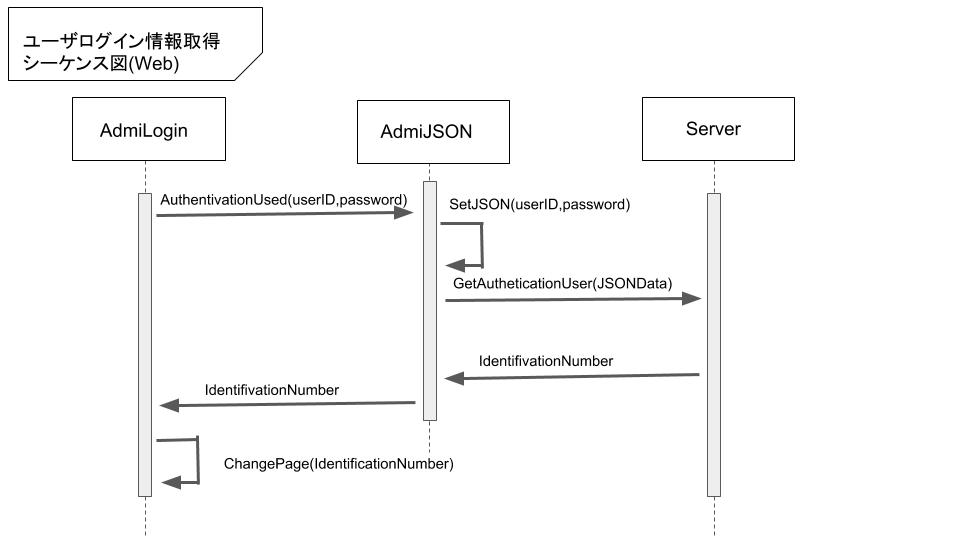
\includegraphics{oonishi1.jpg}}
\caption{ログイン画面ユーザ認証のシーケンス図}
\label{tab:oonishi1}
\end{center}
\end{figure}  
\subsection{店舗情報管理画面店舗登録}
Webの店舗情報管理画面で店舗登録を行う際の相互関係を図 \ref {tab:oonishi2}に示す。
\begin{figure}[H]
\begin{center}
\resizebox{16cm}{!}{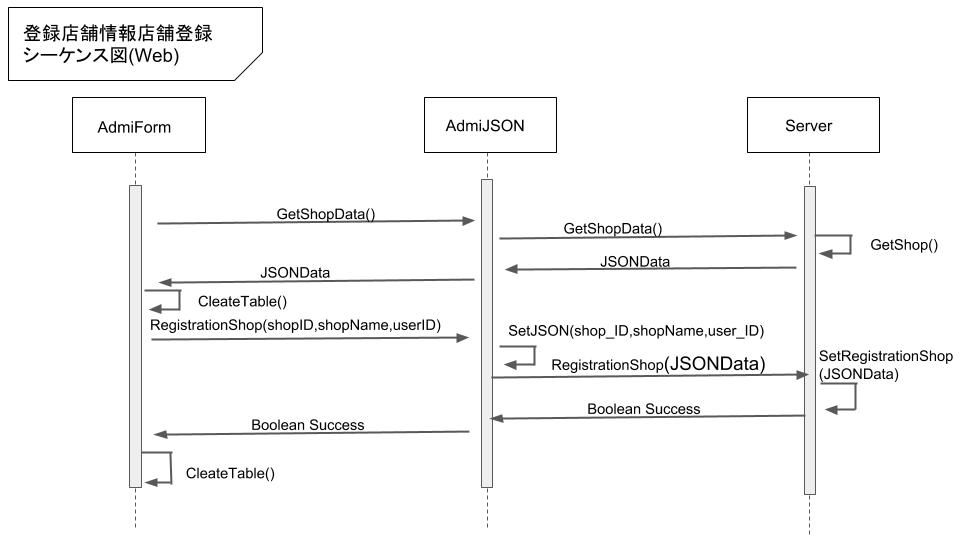
\includegraphics{oonishi2.jpg}}
\caption{店舗情報管理画面店舗登録のシーケンス図}
\label {tab:oonishi2}
\end{center}
\end{figure}
\subsection{店舗情報管理画面店舗更新}
Webの店舗情報管理画面で店長の更新を行う際の相互関係を図 \ref {tab:oonishi3}に示す。
\begin{figure}[H]
\begin{center}
\resizebox{16cm}{!}{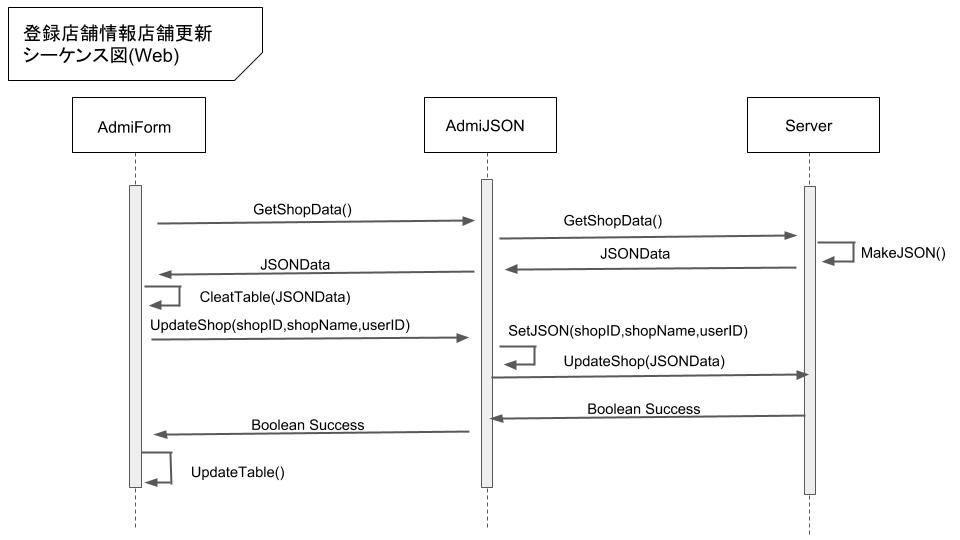
\includegraphics{oonishi3.jpg}}
\caption{店舗情報管理画面店舗更新のシーケンス図}
\label{tab:oonishi3}
\end{center}
\end{figure}
\subsection{店舗情報管理画面店舗削除}
Webの店舗情報管理画面で店舗削除を行う際の相互関係を図 \ref {tab:oonishi4}に示す。
\begin{figure}[H]
\begin{center}
\resizebox{16cm}{!}{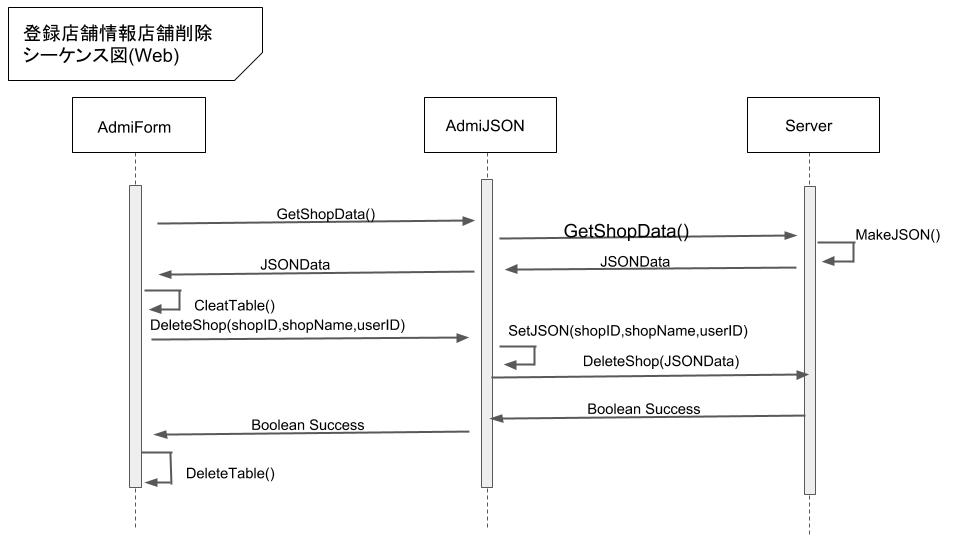
\includegraphics{oonishi4.jpg}}
\caption{店舗情報管理画面店舗削除のシーケンス図}
\label{tab:oonishi4}
\end{center}
\end{figure}

\subsection{特売情報管理画面特売情報登録}
Webの特売情報管理画面で特売情報登録を行う際の相互関係を図 \ref {tab:oonishi21}に示す。
\begin{figure}[H]
\begin{center}
\resizebox{16cm}{!}{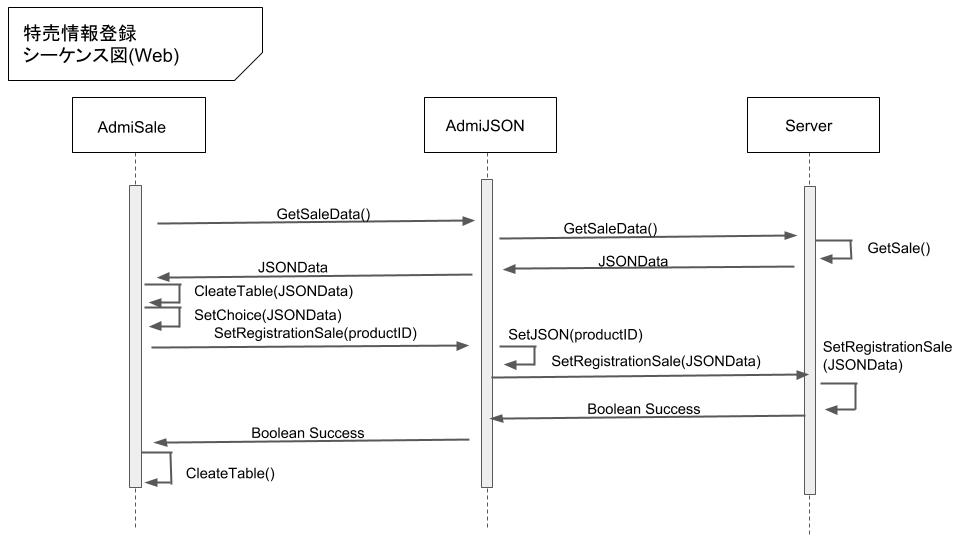
\includegraphics{oonishi21.jpg}}
\caption{特売情報管理画面特売情報登録のシーケンス図}
\label{tab:oonishi21}
\end{center}
\end{figure}
\subsection{特売情報管理画面特売情報削除}
Webの特売情報管理画面で特売情報削除を行う際の相互関係を図 \ref {tab:oonishi22}に示す。
\begin{figure}[H]
\begin{center}
\resizebox{16cm}{!}{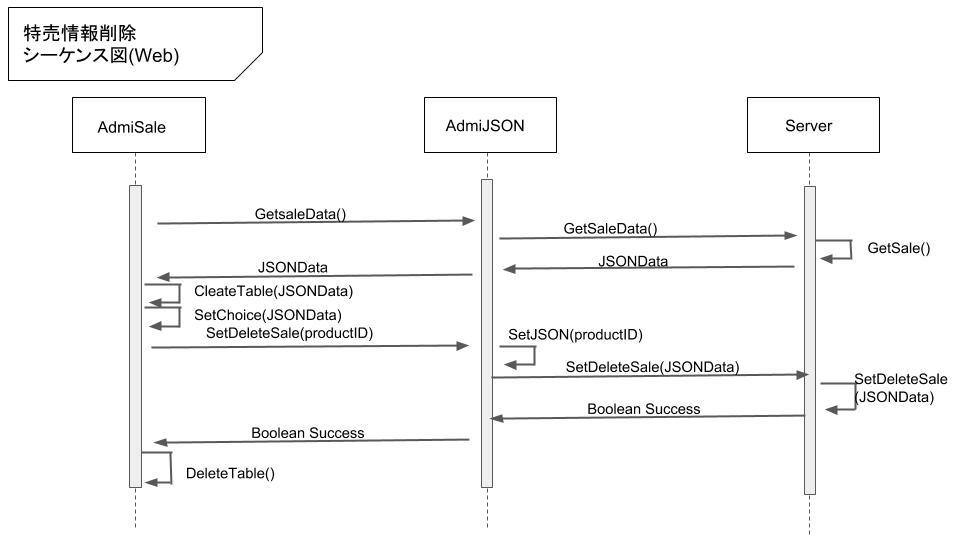
\includegraphics{oonishi22.jpg}}
\caption{特売情報管理画面特売情報削除のシーケンス図}
\label{tab:oonishi22}
\end{center}
\end{figure}
\subsection{特価情報管理画面特価情報登録}
Webの特価情報管理画面で特価情報登録を行う際の相互関係を図 \ref {tab:oonishi23}に示す。
\begin{figure}[H]
\begin{center}
\resizebox{16cm}{!}{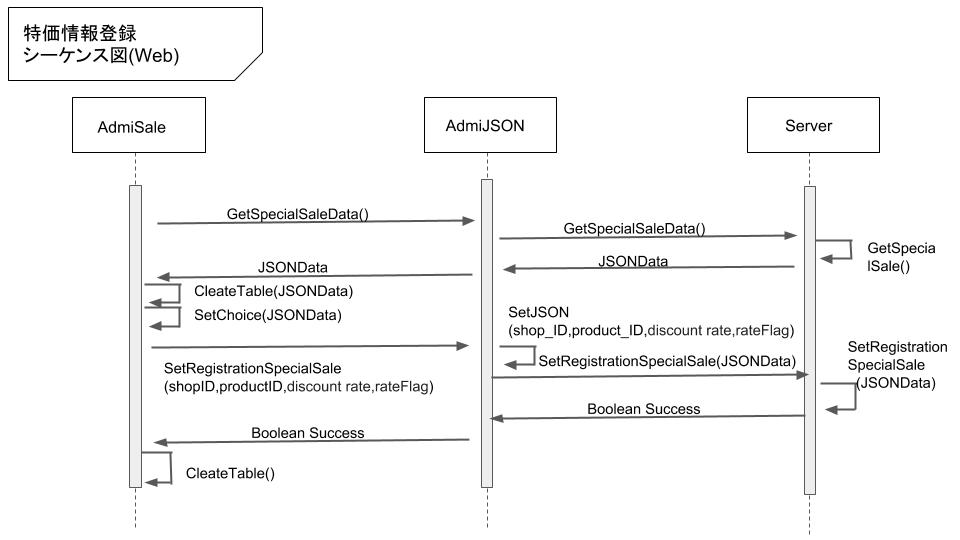
\includegraphics{oonishi23.jpg}}
\caption{特売情報管理画面特売情報登録のシーケンス図}
\label{tab:oonishi23}
\end{center}
\end{figure}
\subsection{特価情報管理画面特価情報更新}
Webの特価情報管理画面で特価情報更新を行う際の相互関係を図 \ref {tab:oonishi24}に示す。
\begin{figure}[H]
\begin{center}
\resizebox{16cm}{!}{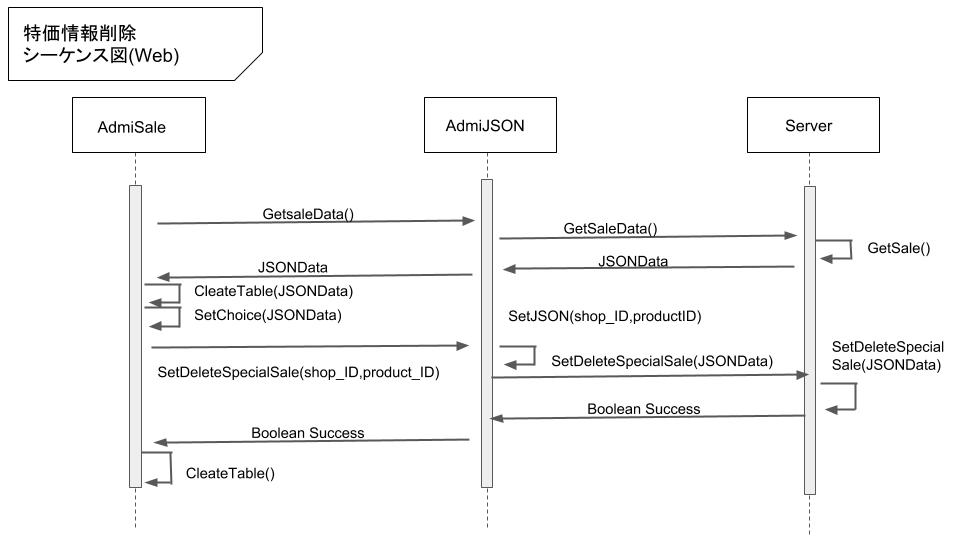
\includegraphics{oonishi24.jpg}}
\caption{特売情報管理画面特売情報更新のシーケンス図}
\label{tab:oonishi24}
\end{center}
\end{figure}
\subsection{特価情報管理画面特価情報削除}
Webの特価情報管理画面で特価情報削除を行う際の相互関係を図 \ref {tab:oonishi25}に示す。
\begin{figure}[H]
\begin{center}
\resizebox{16cm}{!}{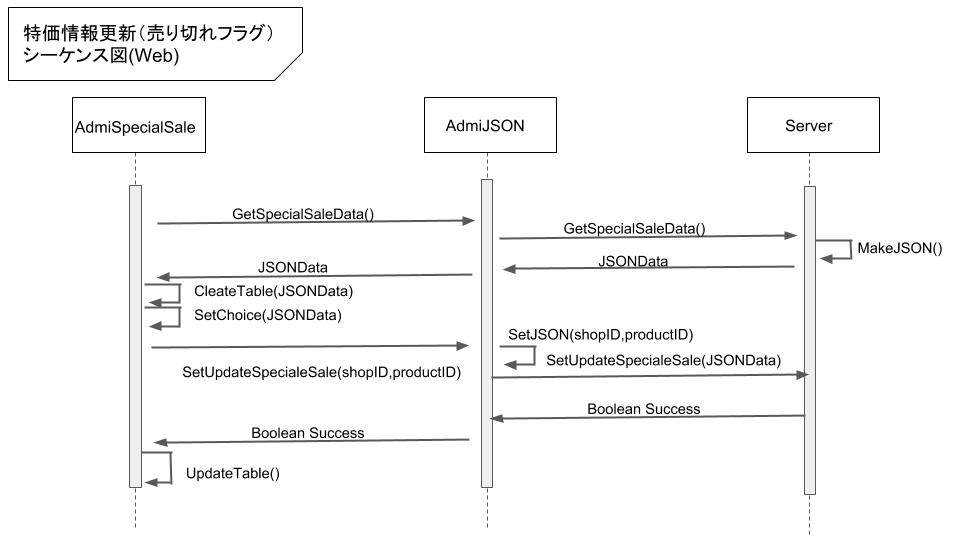
\includegraphics{oonishi25.jpg}}
\caption{特売情報管理画面特売情報削除のシーケンス図}
\label{tab:oonishi25}
\end{center}
\end{figure}
\end{document}